\documentclass[answers]{exam}
\usepackage[utf8]{inputenc}
\usepackage[english]{babel}
\usepackage{amsmath}
\usepackage{mathtools, amsthm}
\usepackage{amsfonts}
\usepackage{amssymb}
\usepackage{mathrsfs}
\usepackage{tcolorbox}


\newtheorem{theorem}{Theorem}[section]
\newtheorem{corollary}{Corollary}[theorem]
\newtheorem{lemma}[theorem]{Lemma}
\renewcommand{\qedsymbol}{$\blacksquare$}
\begin{document}
    %% \union - Example: \union{j \in J}{A_j}
\newcommand{\union}[2]{\underset{#1}\bigcup #2}

%% \inter - like \union, but with \bigcap
\newcommand{\inter}[2]{\underset{#1}\bigcap #2}
    Submitted by: Nutan Nepal
    \begin{questions}

        \begin{minipage}{.69\textwidth}
            \question{
            The given diagram consists of a square of length
            10 cm and arcs of four circle of radius 10 cm.
            Find the area of the largest circle which can be fit
            into the shaded region.
        }
        
        \end{minipage}
        \begin{minipage}{.26\textwidth}
            \begin{flushright}
                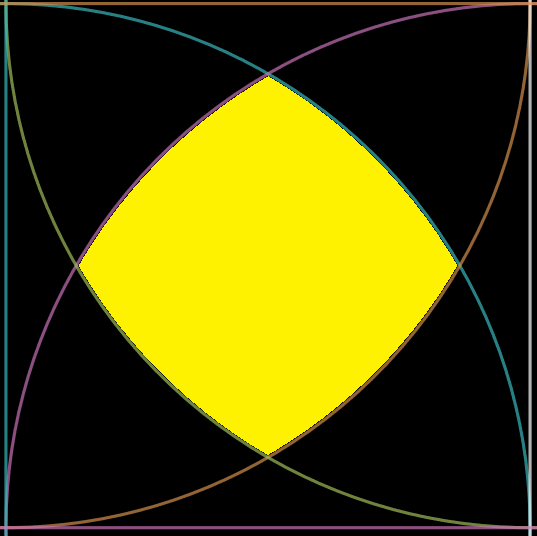
\includegraphics[width=1.5in]{questionmath.PNG}
            \end{flushright}
        \end{minipage}

        \begin{solution}

            \begin{minipage}{.69\textwidth}
            Since the diagonal of the square is $10\sqrt{2}$ cm and
            the radius of each circle is 10 cm, we find that the
            maximal radius $r=10 -\frac{10}{\sqrt{2}}
            =10-5\sqrt{2}$. So the area of the required circle
            is $A=\pi r^2=\pi (10-5\sqrt{2})^2 = 26.95 \text{ cm}^2$.
            \qed
            \end{minipage}
            \begin{minipage}{.3\textwidth}
                \begin{flushright}
                    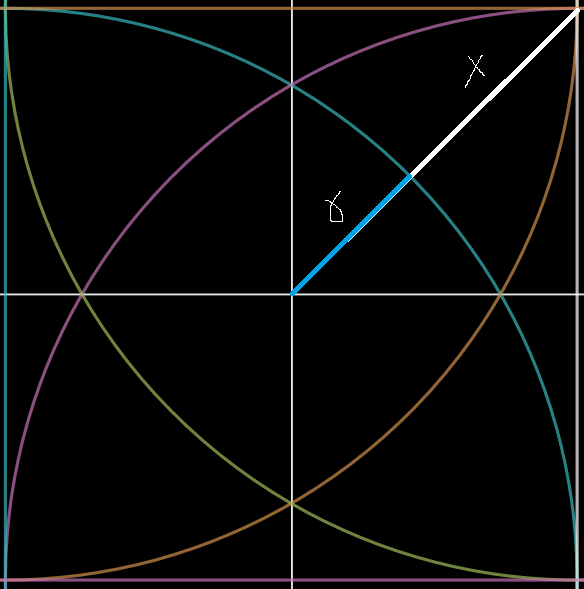
\includegraphics[width=1.5in]{questionmath125.PNG}
                \end{flushright}
            \end{minipage}
        \end{solution}
    \end{questions}
\end{document}